\chapter{Thermal stability of superconducting solenoids}
~~~~~~Radiation will not only genarate the heat inside the coils but also cause the damage of superconducting material, which is possible to lead the degradation of cooling strip.
Due to the conduction cooling, the consequence of aluminum strip degradation is over-heat and quench, which are the major issue for COMET superconducting magnets.
Here, the thermal property of the most dangerous coil, CS1 coil, is analysed.

\section{Quench estimation}
~~~~~Quench plays a significant role in superconducting magnet performance.
Since over 2000 A current is flowing inside the superconducting wire, the resistance of NbTi will increase suddenly when superconducting state turns to the normal state.
If this current cannot decay quickly, the quenching temperature will increase highly and cause the unrecoverable burn-out of superconducting wire.

In Sep. 2008, the accident caused by quench occurred in LHC superconducting magnet.
As the consequence, the bus bar is burned out in the interconnect.
It costs half year to fix the superconducting magnet in LHC accident.
As for the COMET experiment, it is not possible to do the maintenance during the experiment due to the residual radiation of the solenoid.
Thus, the quench estimation is necessary to know the temperature after magnet quenched.

One parameter called MIITs is estimated for the worst situation of quench.
To calculate the MIITs, the specific heat and thermal conductivity from cryogenic temperature to room temperature is required.
The specific heat and electrical resistivity of copper, aluminum and NbTi are fitted with experimental data correctly.

\subsection{Specific heat}
~~~~~There are two models for lattice specific heat, the Debye model and Einstein model~\cite{kittle}.
In Debye model, the phonon energy is written as
\begin{equation}
 U = \int d\omega D(\omega) (\frac{\hbar \omega}{e^{\hbar \omega / \tau}-1})
\end{equation}
where $D(\omega)$ is the density of state, $\omega$ is the wave number.
The desity of state is described as $V\omega^2/2\pi^2v^3$, than the specific heat can be solved as
\begin{equation}
 C_V = \frac{\partial U}{\partial T} = 9 N k_B (\frac{T}{\theta})^3 \int^{x_D}_{0} dx \frac{x^4 e^x}{(e^x-1)^2}
\end{equation}
where $\theta$ is the Debye temperature and equals to $\frac{\hbar v}{k_B} \cdot (\frac{6\pi^2 N}{V})^{1/3}$.
$x_D$ comes from the cut off wave number and equals to $\theta/T$.
%The Debye model can only be used in the range from 0 to $\omega_D$.
In the cryogenic temperature which is less than the Debye temperature ($T\ll\theta$), The specific heat can be approach as
\begin{equation}
 C_V \cong \frac{12 \pi^4}{5} N k_B (\frac{T}{\theta})^3
\end{equation}
Debye model describes the contribution of lattice on specific heat.
However, the contribution of electrons is treated approximately as the free-electron model.
The electronic contribution to specific is
\begin{equation}
 C_V = \gamma T = \frac{1}{2} \pi^2 N k_B \frac{T}{T_F}
\end{equation}
where $\gamma = \pi^2 D(\epsilon_F)k_B^2/3$ is called the Sommerfeld constant and $T_F$ is the Fermi temperature, respectively.
Combining the lattice and electronic contribution, the specific heat can be written as
\begin{equation}
 C_V \cong \gamma T + \beta T^3
\end{equation}
As for the aluminum, the Debye temperature is 428 K and the Sommerfeld constant is 1.35 mJ/mol/K$^2$.
However, it does not agree with the experimental data.
Therefore, the specific heat of aluminum is fitted as polynomial function with different range of temperature.
The details is shown in table~\ref{4alsh} and the fitting result is given in figure~\ref{4alsh2}.
The experimental data is given in reference~\cite{aldata}.
The fitting function does not agree with the experimental in the range from 0 K to 2 K.
Because the initial temperature is 4.5 K, it will not affect the calculation here.
  \begin{figure}[H]
   \begin{subfigure}{0.3\textwidth}
    \centering
	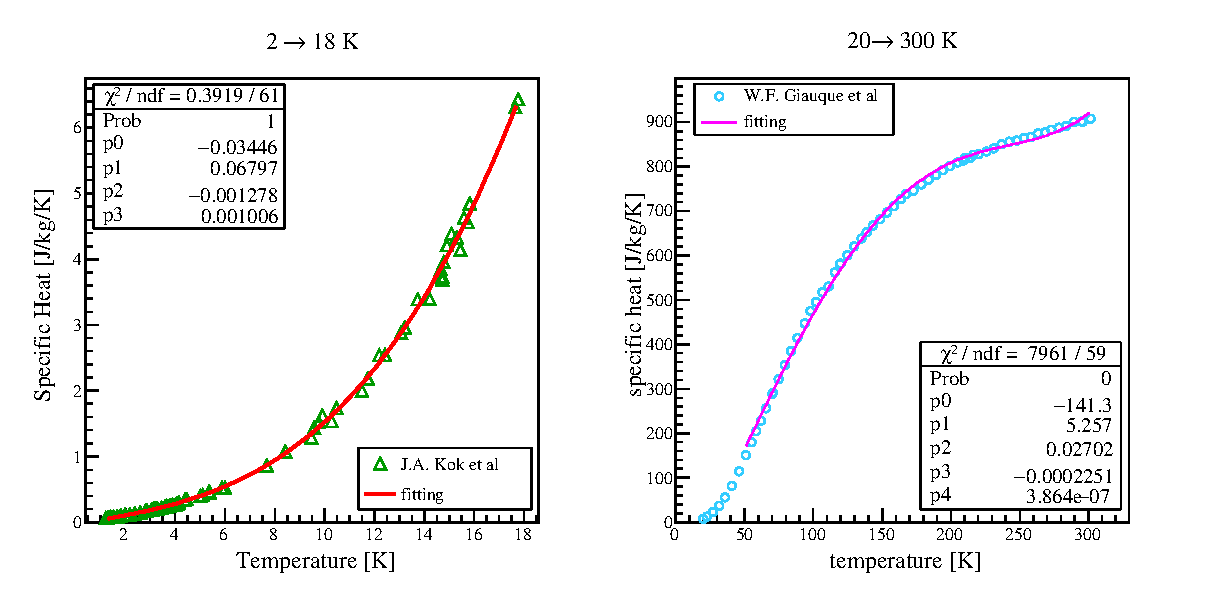
\includegraphics[scale=0.43]{chapter5/fig/alspheat.eps}
   \end{subfigure}
   \hspace{0.2\textwidth}
   \begin{subfigure}{0.3\textwidth}
    \centering
	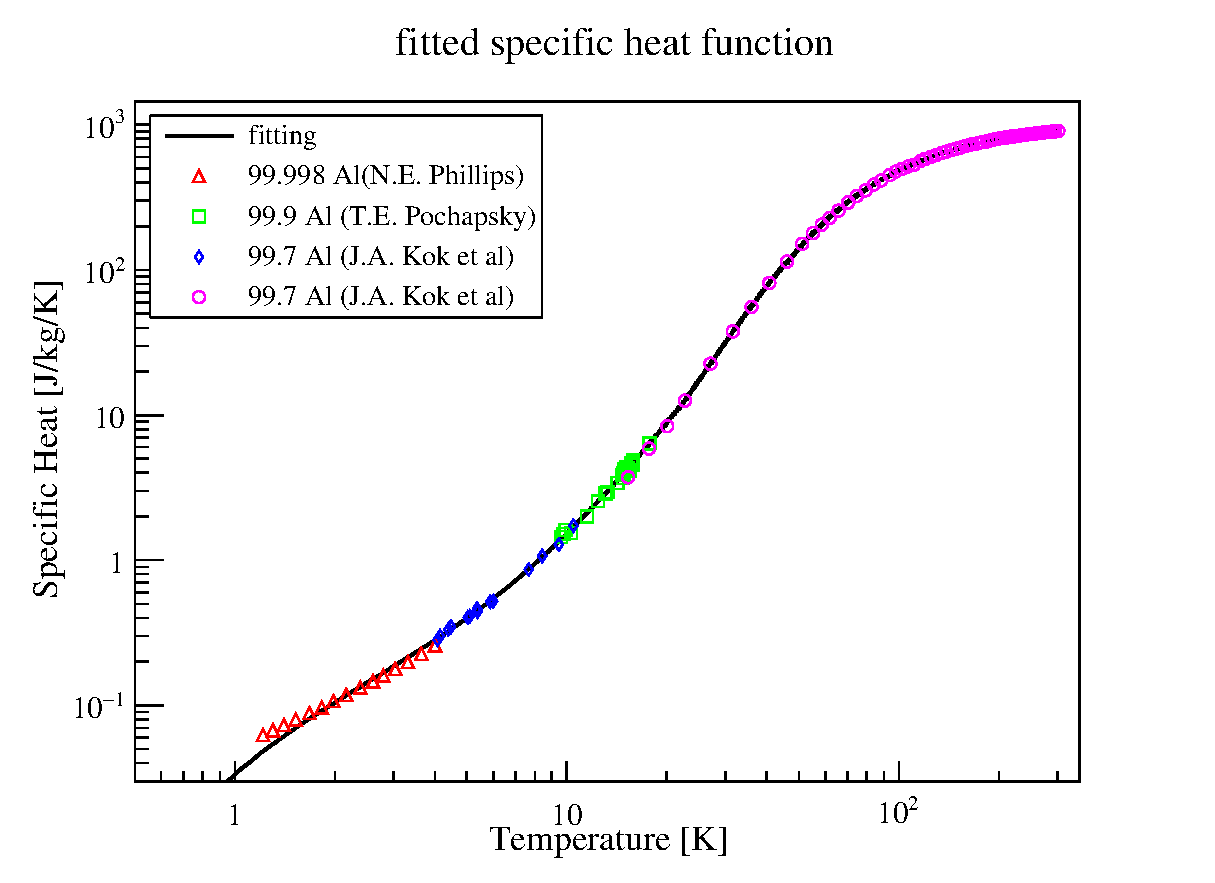
\includegraphics[scale=0.43]{chapter5/fig/alspheat2.eps}
   \end{subfigure}
   \caption{The specific heat of aluminum is fitted from the range from 4.5 K to 22.67 K, 22.67 K to 46 K and 46 K until 350 K respectively.}
   \label{4alsh2}
  \end{figure}
\begin{equation}
 C = p_0 + p_1 \cdot T + p_2 \cdot T^2 + p_3 \cdot T^3
\end{equation}
\begin{table}[H]
 \centering
 \begin{tabular}{cccccc} \hline \hline
 $T_{lower}$ & $T_{upper}$ & $p_0$ & $p_1$ & $p_2$ & $p_3$ \\ \hline
 0 & 22.67 & -0.03446 & 0.06797 & -0.001278 & 0.001006 \\
 22.67 & 46 & 7.88$\times$10$^{13}$ & 6.93201 & -0.07139 & 46.4363 \\
 46 & 350 & 6.273517 & -0.5469 & 0.000925 & -156.932 \\ \hline \hline
 \end{tabular}
 \caption{The details for fitting the aluminum specific heat.}
 \label{4alsh}
\end{table}

The Copper specific heat is fitted as polynomial function with the experimental data in referance~\cite{aldata}.
Here $p_0$ and $p_2 \cdot T^2$ are the correction of specific heat.
$p_1 \cdot T$ and $p_3 \cdot T^3$ are the lattice specific heat and electronic specific heat, respectively.
The fitting parameters are listed in table~\ref{cufit} and the result is shown in figure~\ref{4cush}.
\begin{figure}[H]
   \centering
   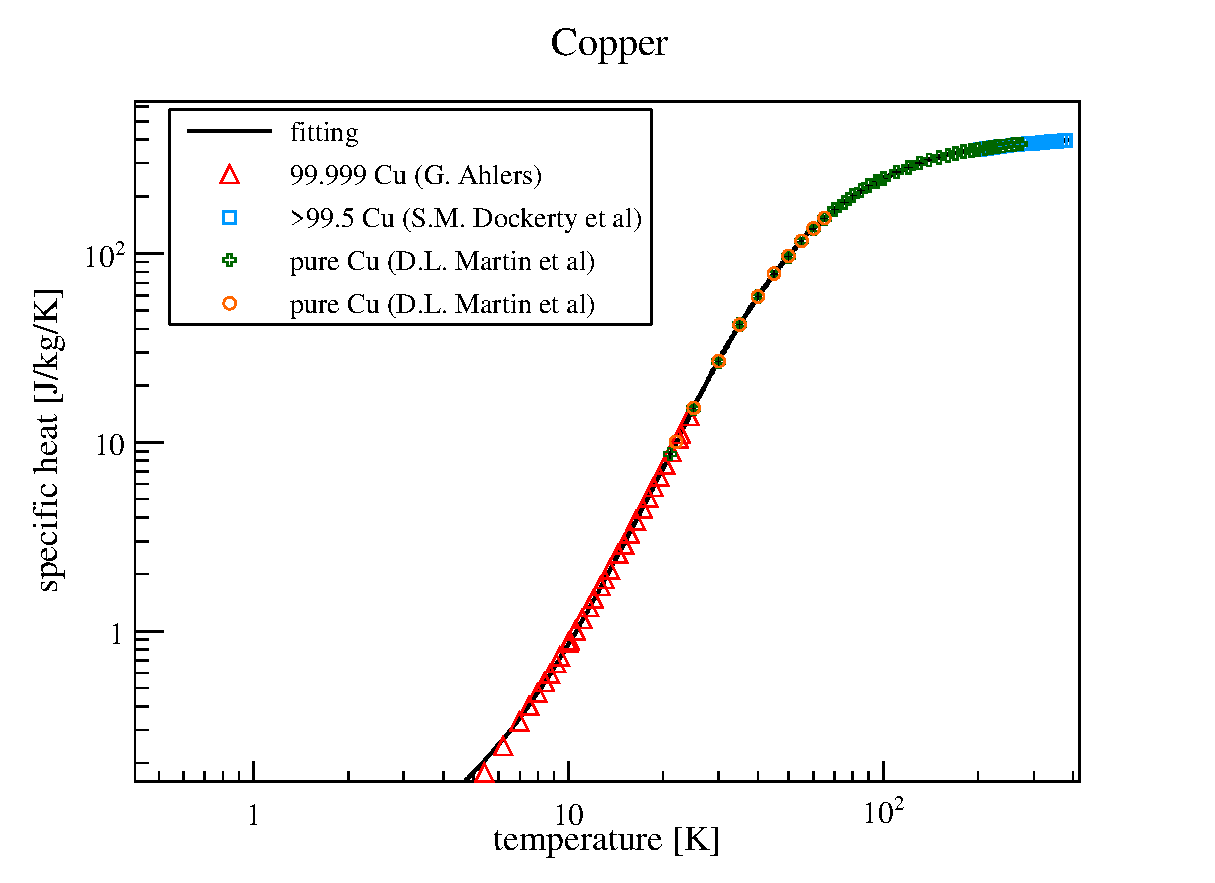
\includegraphics[scale=0.47]{chapter5/fig/cush.eps}
   \caption{ Fitted copper specific heat curve.}
   \label{4cush}
  \end{figure}
\begin{table}[H]
 \centering
 \begin{tabular}{cccccc} \hline \hline
  $T_{lower}$ & $T_{upper}$ & $p_0$ & $p_1$ & $p_2$ & $p_3$ \\ \hline
  0 & 23 & -0.104251 & 0.0832507 & -0.0118811 & 0.00131157 \\
  23 & 55 & 25.2218 & -3.41019 & 0.144053 & -0.000939968 \\
  55 & 250 & -158.094 & 6.40481 & -0.0273429 & 4.08432$\times$10$^{-6}$ \\ \hline \hline
 \end{tabular}
 \caption{Fitting parameters for copper specific heat.}
 \label{cufit}
\end{table}
\begin{table}[H]
 \centering
 \begin{tabular}{ccccccc} \hline \hline
 $T_{lower}$ & $T_{upper}$ & $p_0$ & $p_1$ & $p_2$ & $p_3$ & $p_4$ \\ \hline
 0 & $T_c(B)$ & 0 & 64 $\times$ B & 0 & 49.1 & 0 \\
 $T_c(B)$ & 26.358 & 0 & 928 & 0 & 16.24 & 0 \\
 28.358 & 50.99 & 41383 & -7846.1 & 553.71 & 11.9838 & -0.2177 \\
 50.99 & 165.8 & -1.53$\times$10$^6$ & 83022 & -716.3 & 2.976 & -0.00482 \\
 165.8 & 496.54 & 1.24$\times$10$^6$ & 13706 & -51.66 & 0.09296 & -6.29$\times$10$^{-5}$ \\
 496.54 & 1000 & 2.45$\times$10$^6$ & 955.5 & -0.257 & 0 & 0 \\ \hline \hline
 \end{tabular}
 \caption{The fit parameters for NbTi specific heat.}
 \label{nbtish}
\end{table}
The NbTi specific heat is same to the CUDI parameters which is given in ROXIE's database~\cite{roxie}.
The fit parameters are reported in table~\ref{nbtish}.
\begin{equation}
 C = \rho_{NbTi}\cdot (p_0 + p_1 \cdot T + p_2 \cdot T^2 + p_3 \cdot T^3 + p_4 \cdot T^4)
\end{equation}

  \subsection{Electrical resistivity}
~~~~~~Because of collisions of free electrons with impurities, lattice and phonons, it generates the electrical resistivity.
The electrical resistivity is obtained from the free electron gas model.
\begin{equation}
 \rho = \frac{1}{\sigma} = \frac{m}{ne^2\tau}
\end{equation}

In the room temperature, the collisions of electrons with phonon is dominated the electrical resistivity.
However, only the collisions of electrons with impurities and defects occurs in the cryogenic temperature.
Therefore, the total resistivity can be written as
\begin{equation}
 \rho = \rho_L + \rho_i
\label{reseq}
\end{equation}
where $\rho_L$ is the resistivity from the phonon collisions, $\rho_i$ is the resistivity from the scattering of electron waves with impurities.
$\rho_L$ will become 0 when the temperature is close to 0 K.
There are two ways to fit the electrical resistivity.
\begin{itemize}
 \setlength{\itemsep}{-5pt}
 \item Fit the electrical resistivity directly.
 \item Fit the thermal conductivity first, then covert it with Wiedemann-Franz law.
\end{itemize}

In reference~\cite{nist}, it gives the function to fit the copper electrical resistivity.
Its function contains temperature and RRR dependence like
\begin{equation}
 \rho (T, RRR) = \rho_0 + \rho_i + \rho_{i0}
\end{equation}
$\rho_0$ and $\rho_i$ are same to the two terms in equation~\ref{reseq}, which indicate the resistivity in cryogenic temperature and room temperature, respectively.
$\rho_{i0}$ is the correction term of $\rho_0$ and $\rho_i$
Hence $\rho_0$ depends on the material purity and structure, while $\rho_i$ depends on the temperature.
Each term are given by
\begin{gather}
 \rho_0 = \frac{\rho_{RT}}{RRR} \\
 \rho_i = \frac{p_1 \cdot T^{p_2}}{1 + p_1 \cdot p_3 \cdot T^{(p_2-p_4)} \cdot exp\{-(\frac{p_5}{T})^{p_6}\}} \\
 \rho_{i0} = p_7 \cdot \frac{\rho_i \cdot \rho_0}{\rho_i + \rho_0}
\end{gather}
As for the copper, the electrical resistivity at room temperature is 1.553$\times$10$^{-8}$ [$\Omega\cdot m$], and the same fitting parameters is employed in MIITs simulation which is listed in table~\ref{cures}.
\begin{table}[H]
 \centering
 \begin{tabular}{ccccccc} \hline \hline
  $p_1$ & $p_2$ & $p_3$ & $p_4$ & $p_5$ & $p_6$ & $p_7$ \\ \hline
  1.171$\times$10$^{-17}$ & 4.49 & 3.841$\times$10$^{10}$ & 1.14 & 50 & 6.428 & 0.4531 \\ \hline \hline
 \end{tabular}
 \caption{NIST fitting parameters for copper electrical resistivity.}
 \label{cures}
\end{table}
On the other hand, the electrical resistivity is able to be achieved from the thermal conductivity.
Reference~\cite{wood} mentions the predicting of thermal conductivity which based on a set of semi-empirical equations presented by Hust et al.~\cite{hust}.
The thermal conductivity is written as
\begin{equation}
 K = \frac{1}{W_0 + W_i + W_{i0}}
\end{equation}
where $W_0$ and $W_i$ represent the electron-defect and eletron-phonon interactions respectively, which is similar to the NIST equation.
$W_{i0}$ is necessary to produce acceptable fits.
Each term is given as follows.
\begin{gather}
 W_0 = \frac{\beta}{T} \\
 W_i = \frac{p_1 \cdot T^{p_2}}{1 + p_1p_3T^{(p_2+p_4)}exp\{-(\frac{p_5}{T})^{p_6}\}} + W_c \\
 W_{i0} = p_7 \cdot \frac{W_i W_0}{W_i + W_0}
\end{gather}
The parameter $\beta$ is the function of the residual resistivity $\rho_0$, which can be represented as Wiedemann-Franz law.
\begin{equation}
 \beta = \frac{\rho_0}{L_0} = \frac{\rho_{RT}}{L_0} \cdot \frac{1}{RRR}
\end{equation}
The $W_c$ is correction parameter for only the pure aluminum which is compared with experimental data.
\begin{equation}
 W_c = -0.0005 \cdot ln(\frac{T}{330}) \cdot exp\{-(\frac{ln(T/380)}{0.6})^2\} -0.0013 \cdot ln(\frac{T}{110}) \cdot exp\{-(\frac{ln(T/94)}{0.5})^2\}
\end{equation}

As for the pure aluminum, the fitting parameter for NIST and Hust equation is listed in table~\ref{paraAl} and \ref{paraAl2} respectively.
  \begin{figure}[H]
   \begin{subfigure}{3.1in}
	\centering
    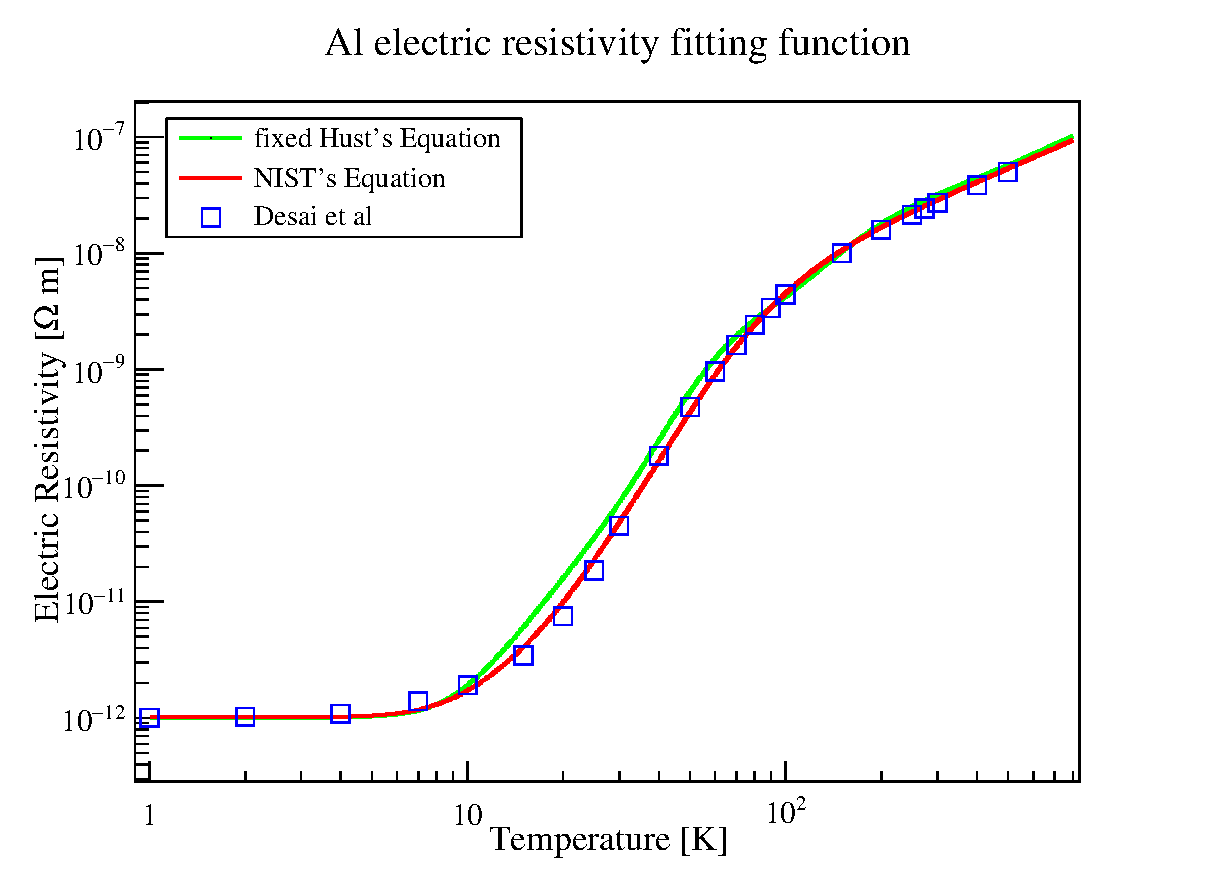
\includegraphics[scale=0.45]{chapter5/fig/alres1.eps}
	\caption{Fixed the Hust's equation and NIST's equation of aluminum electric resistivity.}
    \label{4alres}
   \end{subfigure}
   \quad
   %\hspace{1in}
   \begin{subfigure}{3.1in}
    \centering
    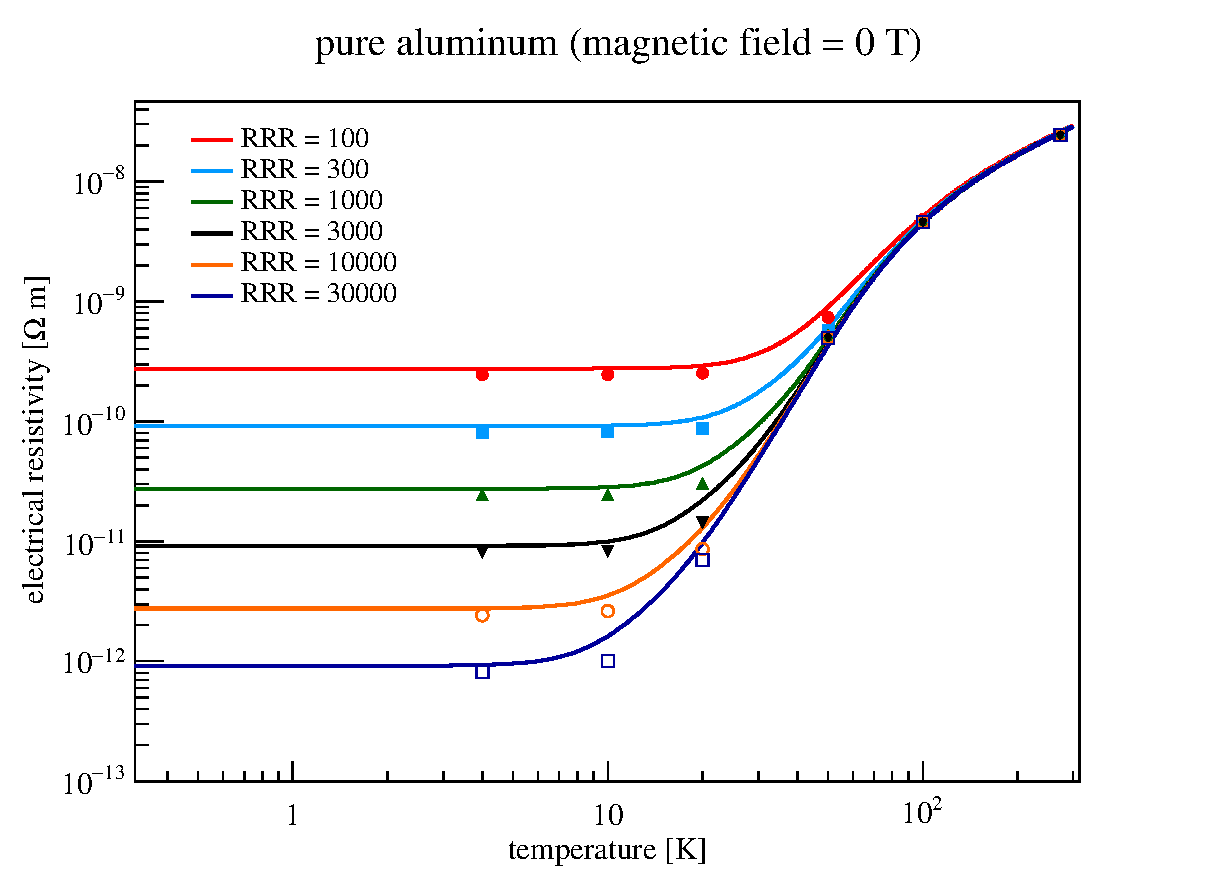
\includegraphics[scale=0.45]{chapter5/fig/resist.eps}
	\caption{Comparison of the aluminum electric resistivity with different RRR.}
    \label{4alres2}
   \end{subfigure}
   \caption{Fitted aluminum resistivity.}
  \end{figure}

\begin{table}[H]
 \centering
 \begin{tabular}{ccccccc} \hline \hline
  $p_1$ & $p_2$ & $p_3$ & $p_4$ & $p_5$ & $p_6$ & $p_7$ \\ \hline
  1.671$\times$10$^{-17}$ & 4.36 & 2.841$\times$10$^{10}$ & 1.18 & 64 & 4.428 & 1.2031 \\ \hline \hline
 \end{tabular}
 \caption{NIST fitting parameter for pure aluminum.}
 \label{paraAl}
\end{table}
\begin{table}[H]
 \centering
 \begin{tabular}{ccccccc} \hline \hline
  $p_1$ & $p_2$ & $p_3$ & $p_4$ & $p_5$ & $p_6$ & $p_7$ \\ \hline
  4.716$\times$10$^{-8}$ & 2.446 & 623.6 & -0.16 & 130.9 & 2.5 & 0.8168 \\ \hline \hline
 \end{tabular}
 \caption{Hust fitting parameter for pure aluminum.}
 \label{paraAl2}
\end{table}
Figure~\ref{4alres} shows the comparsion of the Hust and NIST equation with experimental data by using these fitting parameters for pure aluminum (RRR = 10000)~\cite{desai}.
The fixed Hust equation is higher than the experimental data in the range from 10 K to 100 K.
Hence the Hust equation still needs to be fixed in future.

In figure~\ref{4alres}, only the aluminum with 10000 of RRR is compared to the fitting function.
While, the pure aluminum with different RRR must be agreed to the fitting function and it is shown in figure~\ref{4alres2}.
(The experimental data is obtained from Prof. Nakamoto.)
The fixed NIST equation is employed in here.
The fitting function is higher than experimental data about factor 0.2, and its difference is only shown in low temperature.
As for the high temperature, it has good agreement with data.

  \subsubsection{Magnetoresistivity}
~~~~~Due to the external magnetic field, the mean free path will be shortened and the collisions between eletrons and phonon is increased, which leads to the electrical resistivity increasing.
The Kohler's plot is the most common expression of the magnetoresistvity.
The Corruccini~\cite{corr} gives the equation to calculate the magnetoresistivity in reference~\cite{fick}~\cite{arp}.
The electrical resistivity in the high field can be written as
\begin{gather}
 \rho(B, T) = \rho(0, T) + \rho(0, T) \cdot \frac{h^2 \cdot (p_0 + p_1 \cdot h)}{p_2 + p_3\cdot h + p_4 \cdot h^2} \\
 h = B \cdot \frac{\rho_{ref}}{\rho(0, T)} \cdot 10
\end{gather}
\begin{figure}[H]
 \centering
 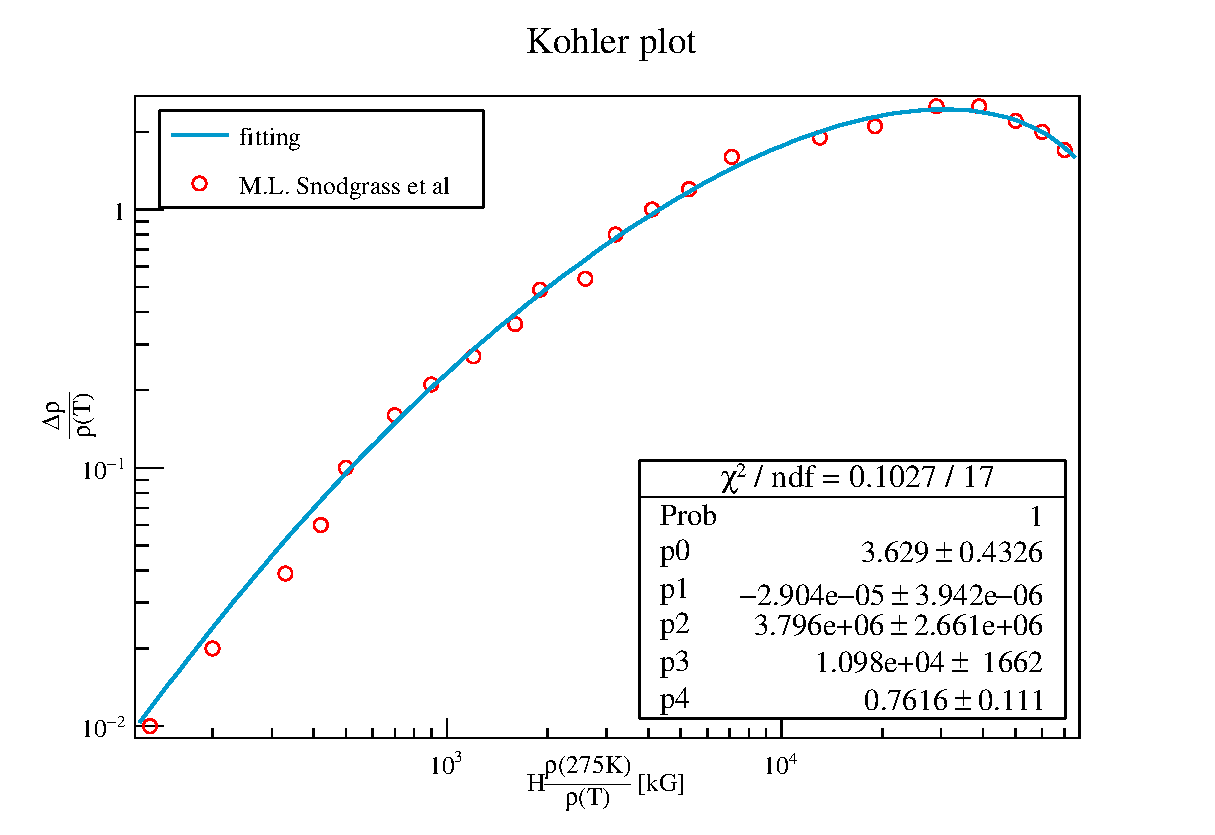
\includegraphics[scale=0.45]{chapter5/fig/Magnetores.eps}
 \caption{Fitted the Kohler plot with experimental data for pure aluminum.}
 \label{4magres}
\end{figure}
where $\rho_{ref}$ is 2.75$\times$10$^{-8}$ [$\Omega\cdot m$] and $\rho(0, T)$ is the eletrical resistivity without magnetic field.
As for the aluminum, the fitting parameters are list in table~\ref{almag} and the fitted Kohler plot is shown in figure~\ref{4magres}.
\begin{table}[H]
 \centering
 \begin{tabular}{ccccc} \hline \hline
  $p_0$ & $p_1$ & $p_2$ & $p_3$ & $p_4$ \\ \hline
  3.62857 & -2.90419$\times$10$^{-5}$ & 3.79649$\times$10$^6$ & 10975.9 & 0.761609 \\ \hline \hline
 \end{tabular}
 \caption{Fitting parameters for pure aluminum magnetorestivity.}
 \label{almag}
\end{table}

As for the copper, the same fitting equation for copper magnetoresistivity in ROXIE is employed in here.
It is fitted as the polynomial function which is given as follows.
\begin{gather}
 \rho(B, T) = \rho(0, T) + \rho(0, T) \cdot 10^h \nonumber \\
 h = p_0 + p_1 \cdot log_{10}x + p_2 \cdot (log_{10}x)^2 + p_3 \cdot (log_{10}x)^3 + p_4 \cdot (log_{10}x)^4 \nonumber \\
 x = \frac{1.553\times 10^{-8} \times B}{\rho(0, T)} \nonumber 
\end{gather}
\begin{table}[H]
 \centering
 \begin{tabular}{ccccc} \hline \hline
  $p_0$ & $p_1$ & $p_2$ & $p_3$ & $p_4$ \\ \hline
  -2.662 & 0.3168 & 0.6229 & -0.1839 & 0.01827 \\ \hline \hline
 \end{tabular}
 \caption{Fitting parameters for copper magnetoresistivity.}
 \label{cumag}
\end{table}

\subsection{Thermal conductivity}
~~~~~Thermal conductivity can be obtained from the electric resistivity by using Wiedemann-Franz law, which is written as
\begin{equation}
 k = \frac{L_0 \cdot T}{\rho}
\end{equation}
\begin{figure}[H]
 \centering
 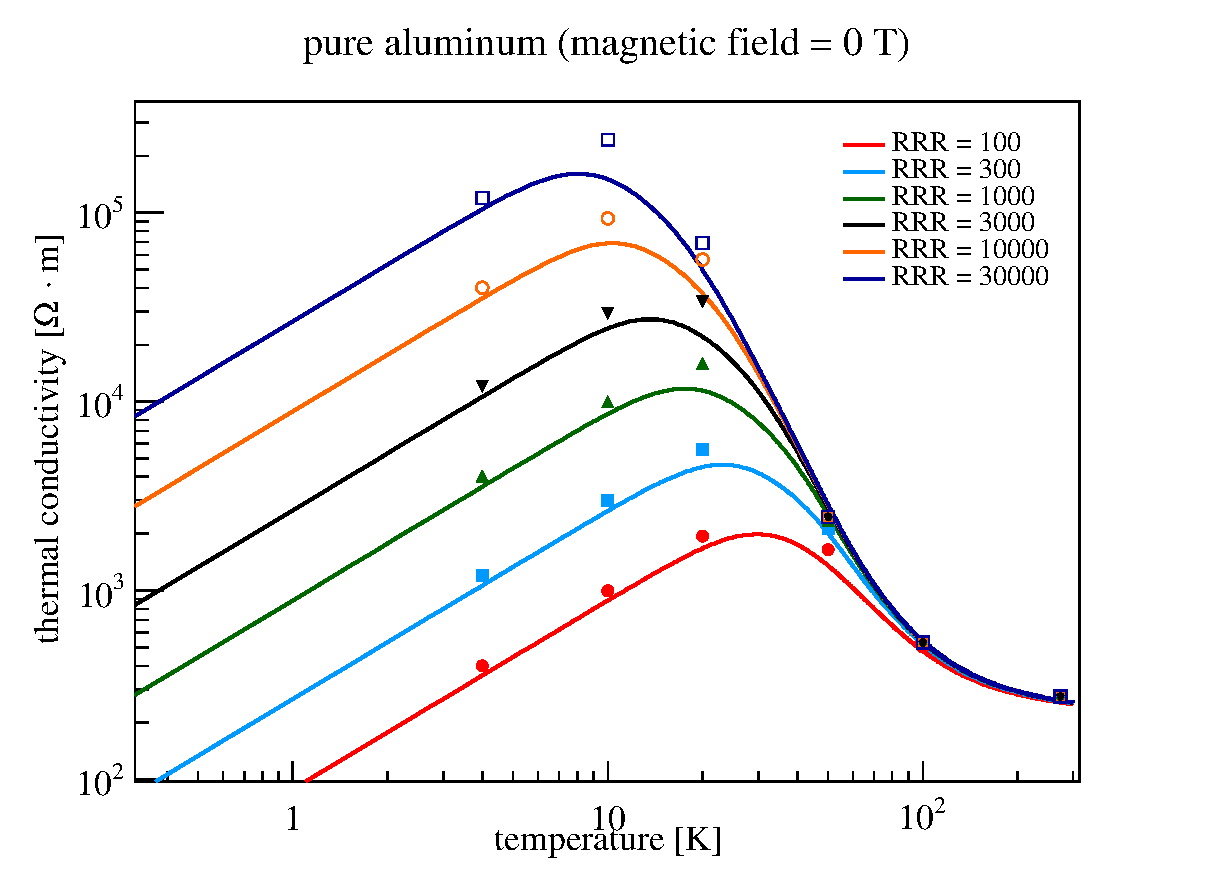
\includegraphics[scale=0.43]{chapter5/fig/thermalcon.eps}
 \caption{Thermal conductivity of aluminum with difference RRR.}
 \label{therm}
\end{figure}
where $\rho$ is the resistivity, and Lorentz constant $L_0$ is defined as
\begin{equation}
 L_0 = \frac{\pi^2}{3}(\frac{k_B}{e})^2 = 2.44\times 10^{-8} W\cdot\Omega /K^2
\end{equation}
The thermal conductivity used in thermal estimation is shown in figure~\ref{therm}.

  \subsection{MIITs}
~~~~~~Because over 2000 A current will generate the joule heat inside the coils, the wire has a risk of burn-out after a quench.
Usually, there is external sump resistor to disspate the stored energy in magnets.
Once the quench has been detected, the power supply will be switched off and the current decays due to the dump resistor.
The current decay can be presented as
\begin{equation}
 I = I_0 \cdot exp(-\frac{R}{L} t)
\end{equation}
where $L$ is the inductance of magnet.
The speed of current decay depends on the inductance and resistance and the current can totally decay in the time of $\tau = L/R$.
The quenching temperature can be restrained if the current decays quickly.

Due to the stored energy is $I^2(t)R(T)$, a relation between the time dependence of the current after quench and the maximum temperature can be established.
The temperature change during the a time interval $dt$ can be written as
\begin{equation}
 dT = \frac{1}{C(T)} R(T) I^2(t) dt
\end{equation}
where specific heat $C(T)$ and resistance $R(T)$ depend on the temperature, and the current $I(t)$ depends on the time.
Seperating and intergrating the time term and the temperature term, one relation can be obtained
\begin{equation}
 f(T_{max}) = \int^{\infty}_0 I^2(t) \cdot dt = \int^{T_{max}}_{T_0} \frac{C(T)}{R(T)} \cdot dT
\end{equation}
The unit of the time integral over the square of the current is usually defined as 10$^6\cdot$A$^2\cdot$sec, which sometimes is called as "MIITs".
As for COMET supercoducting magnet, the conductor consists of NbTi superconducting filament, copper matrix and aluminum stabilizer.
Thus, the specific heat $C(T)$ and resistance $R(T)$ need to average like
\begin{gather}
 C(T) = \gamma_{Cu} \cdot C_{Cu}(T) \cdot A_{Cu} + \gamma_{NbTi} \cdot C_{NbTi}(T) \cdot A_{NbTi} + \gamma_{Al} \cdot C_{Al}(T) \cdot A_{Al} \\
 R(T) = (\frac{A_{Cu}}{\rho_{Cu}(T)} + \frac{A_{Al}}{\rho_{Al}(T)})^{-1}
\end{gather}
where $A$ and $\gamma$ are the cross section and density respectively.
Noting that the unit of $C(T)$ must be [J/K/m$^3$] and the unit of each material's specific heat is [J/K/kg].
The reason why the resistance of NbTi is not included because the resistance of NbTi becomes so high that the current only flows into aluminum stabilizer and copper matrix when quench happens.
The parameters used in MIITs calculation is listed as follows.
\begin{table}[H]
 \centering
 \begin{tabular}{cccccc} \hline \hline
  I$_0$ & R & L & $\tau$ & T$_0$ & Al:Cu:NbTi \\ \hline
  2700 A & 0.185 $\Omega$ & 12.69 H & 68.65 sec & 4.5 K & 7.3:1:1 \\ \hline \hline
 \end{tabular}
 \caption{The parameters for MIITs estimation of CS1.}
 \label{miitspara}
\end{table}
The resistance in table~\ref{miitspara} is the resistance of dump resistor, which is calculated by assuming the allowable voltage of 500 V.
The MIITs curve with 5.5 Tesla for different RRR is shown in figure~\ref{4miits}.
Since the MIITs calculated from time term is 250 MA$^2$sec, the maximum temperature will exceed 260 K if the RRR drops to 100 (90-day continuous operation).
  \begin{figure}[H]
   \centering
   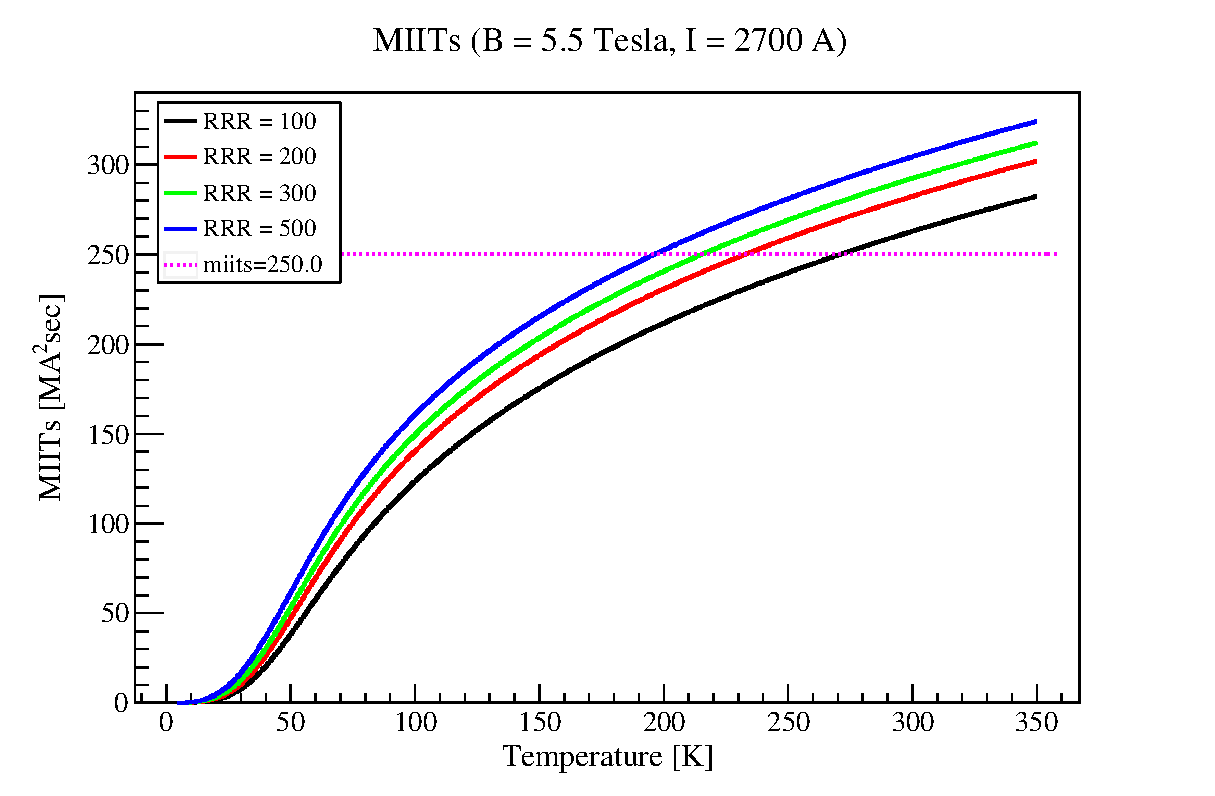
\includegraphics[scale=0.48]{chapter5/fig/I2700.eps}
   \caption{ The MIITs calculation of CS1 coils with 5.5 Tesla magnetic field and 2700 A current.}
   \label{4miits}
  \end{figure}

Figure~\ref{4rrrmiits} shows the prediction of maximum temperature from MIITs in different magnetic field.
Even the magnetic field becomes 0 Tesla, the maximum temperature is still close to 200 K if RRR drops to 100.
Due to the conduction cooling, 200 K is quite high for the superconducting magnets.
Following the temperature increasing, it is possible to lead to the consequence of unstuck insulation tape.
To avoid the overheat after quench, the voltage should be increased.
Figure~\ref{4miitsv} gives the relation between voltage and MIITs predicted maximum temperature.
To reduce the maximum temperature after quench, the MIITs should be restrained under 200 MA$^2$sec and the voltage must be higher than 600 V.
  \begin{figure}[H]
   \begin{subfigure}{3.1in}
    \centering
    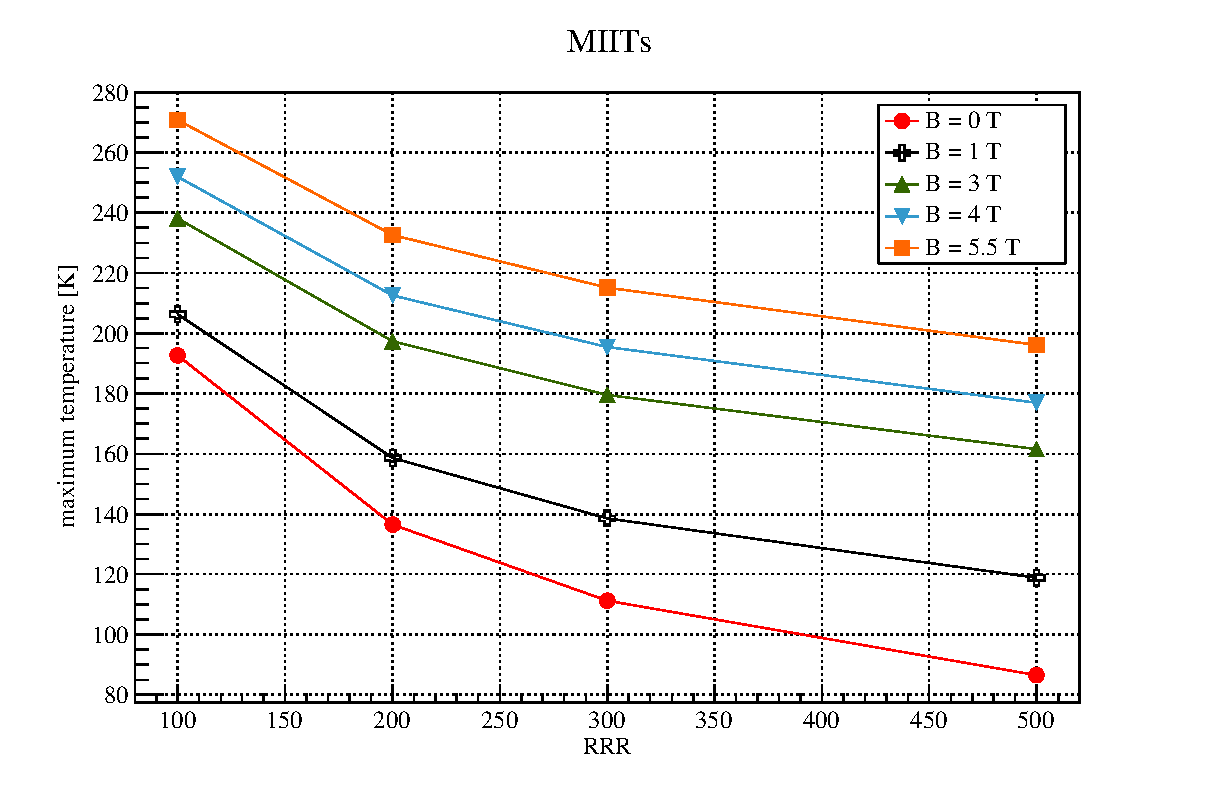
\includegraphics[scale=0.43]{chapter5/fig/RRRvsMIITs.eps}
    \caption{The maximum temperature after magnet quench predicted by MIITs calculation.}
    \label{4rrrmiits}
   \end{subfigure}
   \quad
   \begin{subfigure}{3.1in}
    \centering
    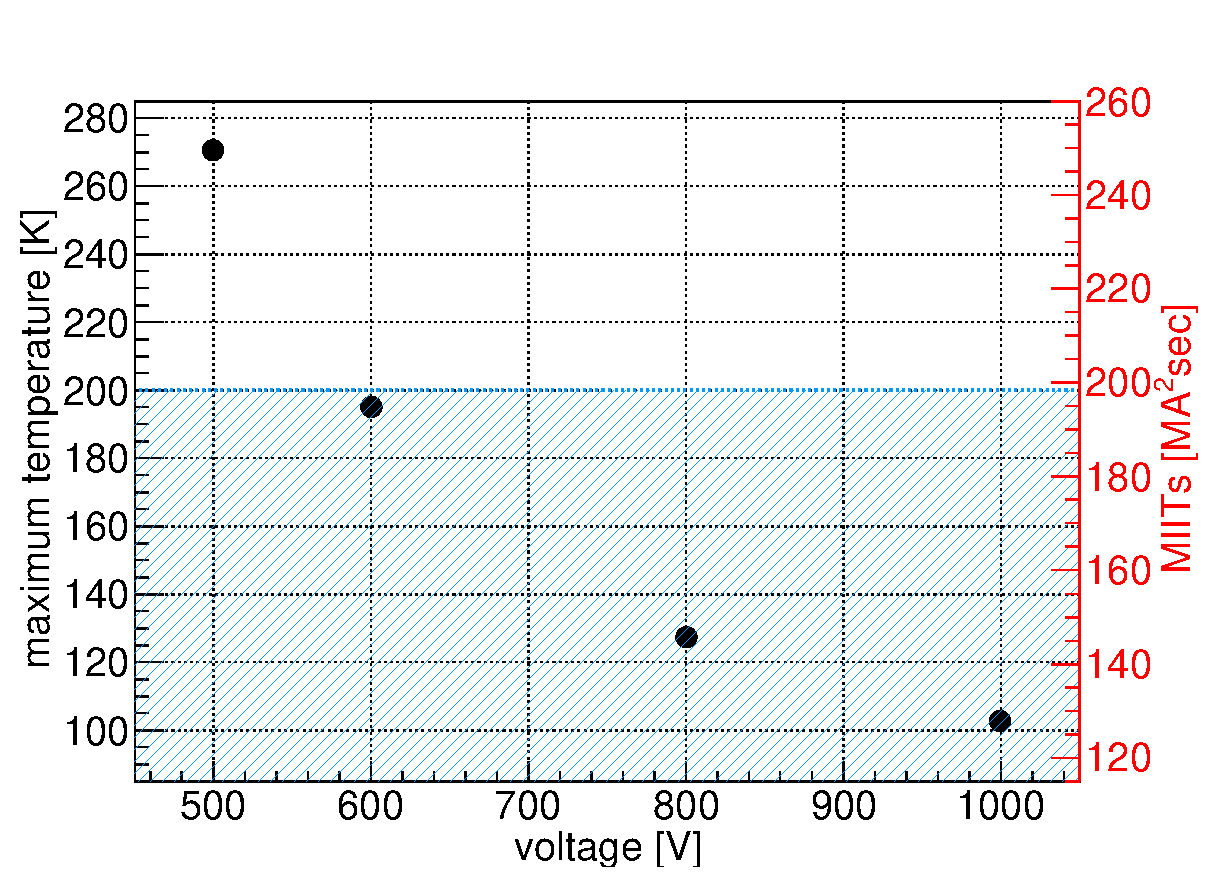
\includegraphics[scale=0.43]{chapter5/fig/miitsvoltage.eps}
    \caption{A relation between voltage and maximum temperature predicted by MIITs.}
    \label{4miitsv}
   \end{subfigure}
   \caption{Improvement of power supply according to the results of MIITs estimation.}
  \end{figure}
However, MIITs can only estimate the maximum temperature of the worst situation.
As the case of COMET superconducting magnets, there are aluminum stabilizer is enclosed around the coils.
The current decay will be more quickly for the real case due to the aluminum stabilizer self resistance.
Furthermore, the magnetic field decay is not considered in MIITs estimation as well.
Thus, the quench simulation is necessary for estimation of the temperature after quench.


 \section{Cooling estimation}
~~~~~~To analyse the thermal stability of superconducting magnet, a thermal simulation code for COMET superconducting magnet has been developed.
This code bases on the three dimensional equation~\cite{heat}, which is written as
\begin{equation}
 \gamma C \frac{dT}{dt} = k_x \frac{\partial^2 T}{\partial x^2} + k_y \frac{\partial^2 T}{\partial y^2} + k_z \frac{\partial^2 T}{\partial z^2} + W
\end{equation}
where $\gamma$, C, k and W are material's density, specific heat, thermal conductivity and heat generation, respectively.
The specific heat only affects the speed of temperature change, and maximum temperature change during the cooling is affected by the term of thermal conductivity and heat generation.
%Due to the Wiedemann-Franz law~\cite{wiede}, the thermal conductivity is converted from electrical conductivity.
%\begin{equation}
% k = \frac{L_0T}{\rho} \\
%\end{equation}
%where $L_0$ is the Lorentz constant, which is 2.45$\times$10$^{-8}$ $W\cdot \Omega/K^2$.
Considering the insulation tape has the worse thermal conductivity, the thermal conductivity of conductor is able to be approached like
\begin{equation}
% \bigtriangleup T = \sum^{\infty}_{i=1} \frac{l_i}{k_i} \cdot \frac{Q}{A} \nonumber \\
 \frac{\sum^{\infty}_{i=1}l_i}{k} = \sum^{\infty}_{i=1} \frac{l_i}{k_i}
\end{equation}
The temperature margin for COMET superconducting magnets can be solved by using the result of energy deposition and neutron flux from PHITS code.

  \subsection{Geometry}
~~~~~~~The geometry which used in thermal analysis is shown in figure~\ref{4geo}.
CS1 coils have 9 layers and 270 turns totally, and aluminum strips with RRR of 2000 are inserted into each layer.
Because there is a GFRP spacer in the edge of each layer, aluminum strips only can be inserted from single side.
Every aluminum is connected to the 2 phase LHe cooling pipe with 4.5 K.
On the top of coils, one aluminum supporter with 5 cm suppresses the coils from hoop stress.
 \begin{figure}[H]
   \begin{subfigure}{0.3\textwidth}
    \centering
    \includegraphics[scale=0.29]{chapter5/fig/geo.pdf}
   \end{subfigure}
   \hspace{0.2\textwidth}
   \begin{subfigure}{0.3\textwidth}
    \centering
	\includegraphics[scale=0.29]{chapter5/fig/geo2.pdf}
   \end{subfigure}
   \caption{Details of the geometry used in magnet thermal simulation.}
   \label{4geo}
  \end{figure}
 
 \subsection{Heat generation}
~~~~~~During the operation, heat generation inside the superconducting magnet is easy to cause the quench of magnet.
Several main heat generations are listed in table~\ref{theat}. 
Thermal radiation is the absorption or emitting of the electromagnetic wave energy.
AC loss is occurred by the alternating magnetic field.
Because the prompt radiation contributes 172.5 W in heat load, the others can be neglected in simulation.
 \begin{table}[H]
  \centering
  \begin{tabular}{cccc} \hline \hline
    & Heat load [W] & & Heat load [W] \\ \hline
	Thermal radiation & 4.16 & Supporter & 4.41 \\
	Current lead & 2.00 & Residual gas & 0.20 \\
	AC loss & 0.50 & Radiation & 172.48 \\ \hline \hline
  \end{tabular}
  \caption{Heat generation for the capture solenoid.}
  \label{theat}
 \end{table}
 \begin{figure}[H]
  \begin{subfigure}{0.25\textwidth}
   \centering
   \includegraphics[scale=0.23]{chapter5/fig/heatgeo1.pdf}
  \end{subfigure}
  \hspace{0.2\textwidth}
  \begin{subfigure}{0.27\textwidth}
   \centering
   \includegraphics[scale=0.23]{chapter5/fig/heatgeo2.pdf}
  \end{subfigure}
  \caption{Mesh cutting of CS1 coils.}
  \label{4geoh}
 \end{figure}
The heat load (energy deposition) is calculated by PHITS code with realistic shielding geometry in figure~\ref{4geoh}.
Superconducting coils consist of NbTi, Al and Cu with 3.80 g/cm$^3$ are cut for 5 parts along the z direction, 4 parts along the azimuthal direction and 9 parts along the radius direction in calculation.
As the result shown in figure~\ref{4heat}, the peak is located on the place 40 cm far from the production target along the z direction, and from 3$\pi$/4 to 5$\pi$/4 along the azimuthal direction.
The energy deposition of inner layer is about 3 times higher than the outer layer's.
 \begin{figure}[H]
  \centering
  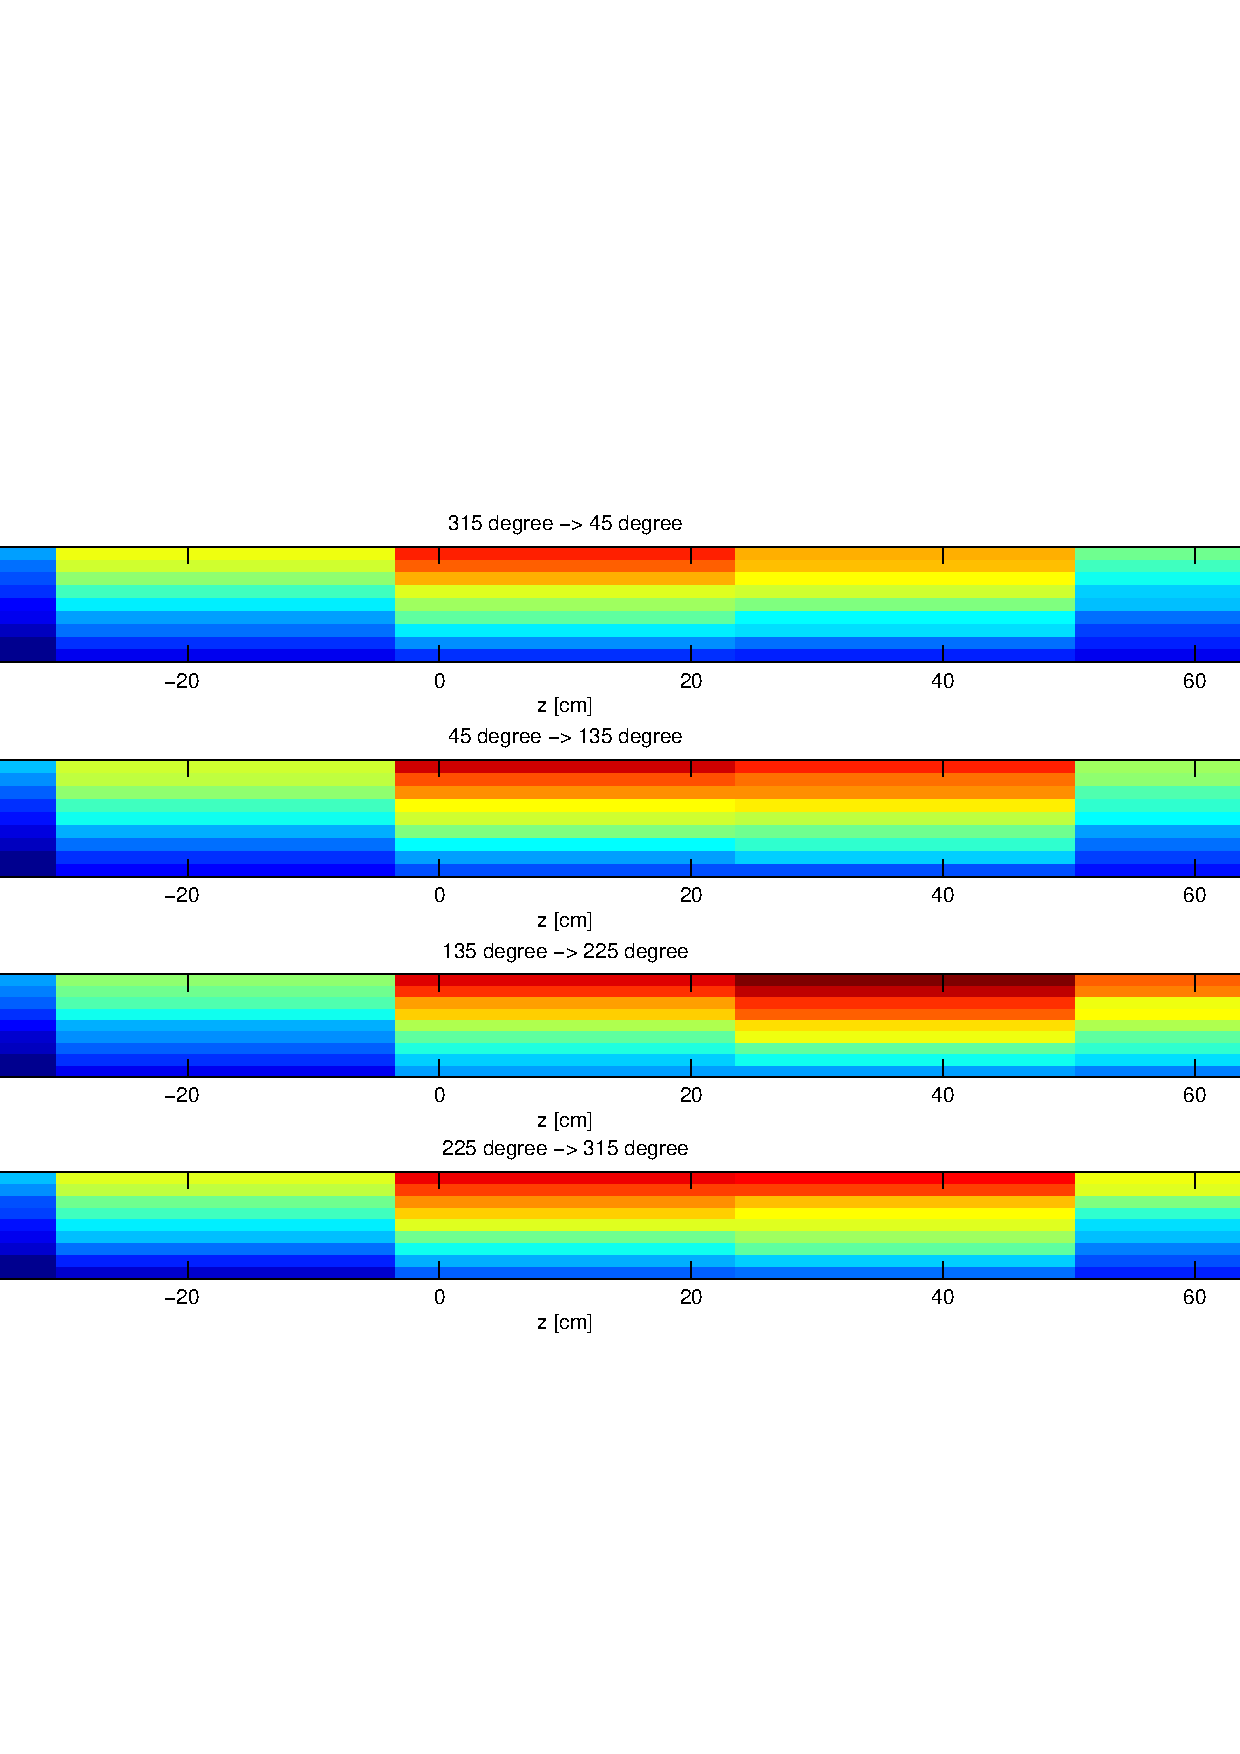
\includegraphics[scale=0.62]{chapter5/fig/HRS.pdf}
  \caption{ Calculated the energy deposition distribution with realistic radiation shield geometry.}
  \label{4heat}
 \end{figure}

  \subsection{Maximum temperature of cooling}
~~~~~~The parameters used in thermal analysis for CS1 coil is listed in table~\ref{para}.
The specific heat only affects the speed of heat transfer and thermal conductivity has no remarkable in range from cryogenic temperature to about 20 K for both copper and aluminum, therefore the specific heat and thermal conductivity are set to constant which does not change with temperature here.
However, the thermal conductivity of insulation tape is still unknown, so it is supposed to 0.01 W/m/K which is worser than Kapton tape.
Its thermal conductivity although depends on the temperature, setting it to one constant is the worst circumstances for CS1 coil.
 \begin{table}[H]
  \centering
  \begin{tabular}{cccc} \hline \hline
   Al strip thickness & 1mm & Conductor cross section & 15 mm $\times$ 4.73 mm \\
   Insulation tape thickness & 0.075 mm $\times$ 2 & Insulation thickness & 0.8 mm \\
   Al:Cu:NbTi & 7.3:1:1 & Supporter shell thickness & 50 mm \\
   End strip to helium & 25 cm & Al density & 2700 kg/m$^3$ \\
   Conductor density & 4000 kg/m$^3$ & Insulation tape desity & 1420 kg/m$^3$ \\
   Tape thermal conductivity & 0.01 W/m/K & Al specific heat & 0.225 J/kg/K \\
   Conductor specific heat & 0.16 J/kg/K & Tape specific heat & 1090 J/kg/K \\ \hline \hline
  \end{tabular}
 \caption{Parameter setting in thermal estimation of CS1 coils.}
 \label{para}
 \end{table}
Due to the finite difference method used in thermal simulation, the result will grow up to infinite if the geometry's mesh and time mesh is not proper in calculation.
Here, as for the issue of meshing, the proper mesh for thermal analysis in this time is founded and listed in table~\ref{4mesh}.
 \begin{table}[H]
  \centering
  \begin{tabular}{ccc} \hline \hline
   Axis & Meshing & Length \\ \hline
   z & 45 & 135 cm \\
   $\phi$ & 4 & 503 cm \\
   r & 19 & 14.4 cm \\
   time & 0.0001 sec & \\ \hline \hline
  \end{tabular}
  \caption{Meshing set in thermal analysis of CS1 coils.}
  \label{4mesh}
 \end{table}
 \begin{figure}[H]
   \begin{subfigure}{0.3\textwidth}
    \centering
	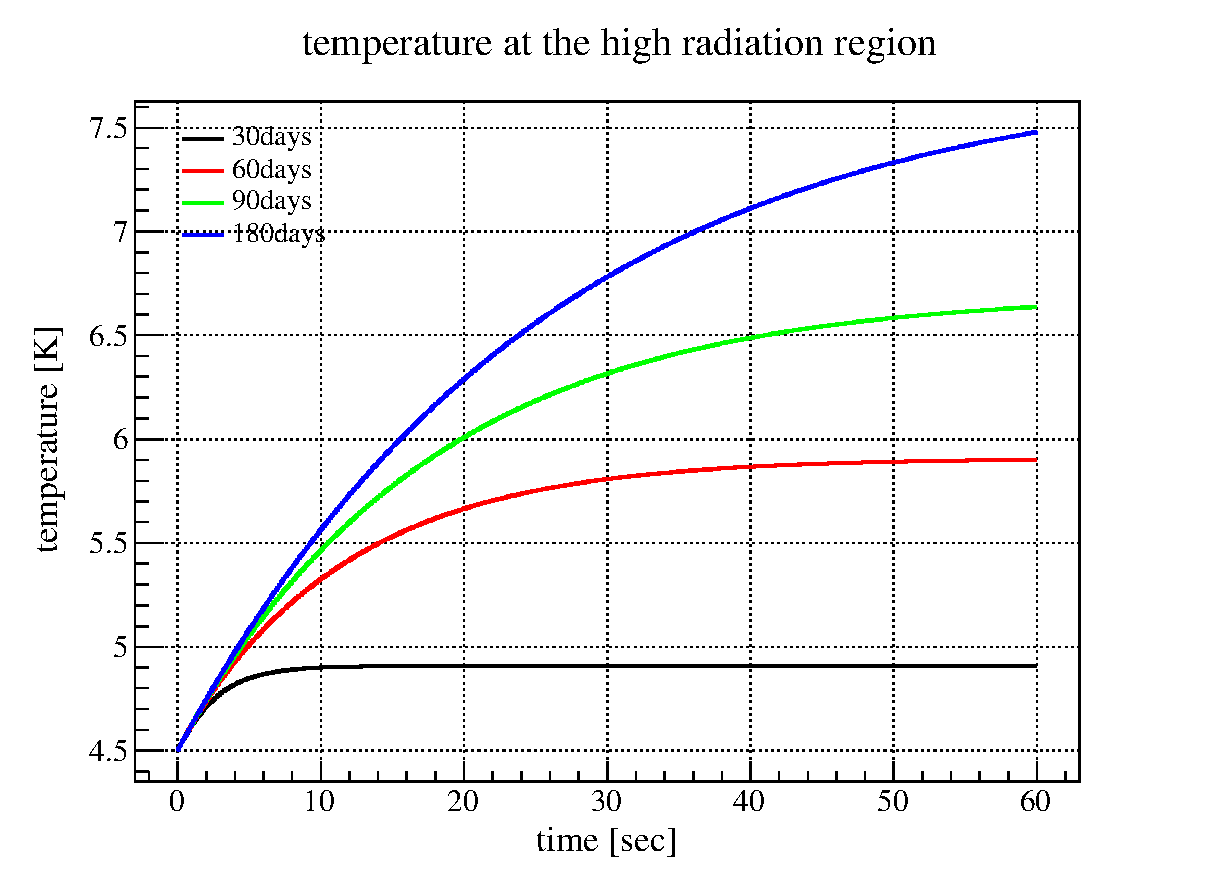
\includegraphics[scale=0.42]{chapter5/fig/time.eps}
   \end{subfigure}
   \hspace{0.2\textwidth}
   \begin{subfigure}{0.3\textwidth}
    \centering
	\includegraphics[scale=0.42]{chapter5/fig/heatdis.pdf}
   \end{subfigure}
   \caption{Calculated the temperature rising during the operation.}
   \label{4heatdis}
  \end{figure}
Superconducting coils have a risk of quench when its temperature closes to the current sharing temperature.
Thus, the peak of temperature must be suppressed under the current sharing temperature for sercuring the coils from quench.
According to K. H. Mess's book, the current sharing temperature is given by
\begin{equation}
 T_{cs} = T_0 + (T_c - T_0)\cdot (1 - \frac{I}{I_c(T_0)})
\end{equation}
where $T_0$ is the initial temperature, $I$ is the operating current, and $I_c(T_0)$ is the critical current in initial temperature.
The current sharing for COMET CS1 coils is 5.6 K (Dr. Sasaki's work).
\begin{figure}[H]
 \centering
 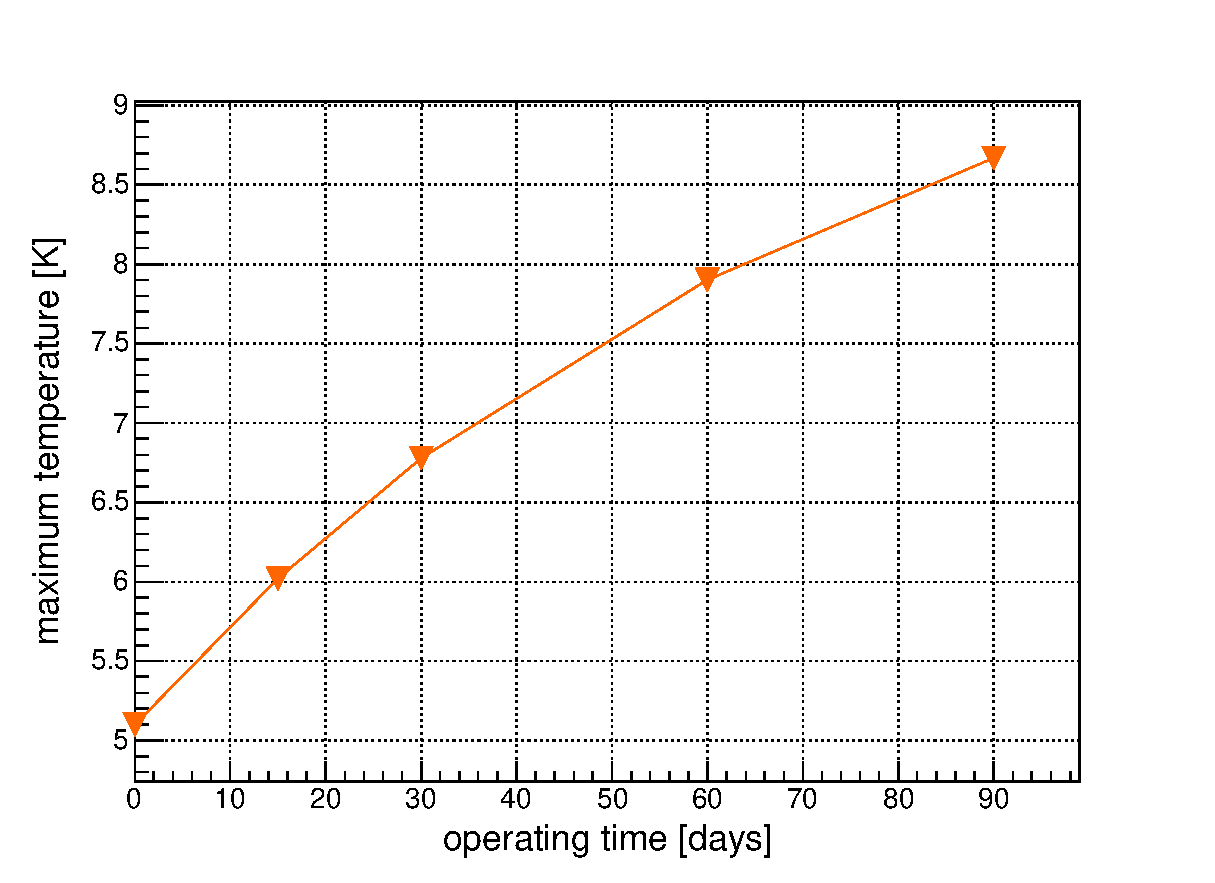
\includegraphics[scale=0.43]{chapter5/fig/temp.eps}
 \caption{ Maximum temperature for the original coil structure.}
 \label{origin}
\end{figure}
Figure~\ref{4heatdis} gives the temperature distribution of 9 layers of conductor and the temperature change with time.
As for figure shown on the left, following the operation time increases, it needs more time to become stable.
The temperature peak is in the middle of CS1 and innermost layer.
Maximum temperature given in figure~\ref{origin} and \ref{4maxtemp} is the peak temperature in CS1 coils.
As for the original design, which shown in figure~\ref{origin}, the peak temperature will reach to the current sharing temperature after 25-day operation.
Considering the simulation uncertainty, only 10-day continuous operation is allowed for phase-II experiment.
Since the superconducting magnet needs almost 1 month to be cooled down to 4.2 K, the plan of 10-day operation wastes a lot of beam time for experiment.
Therefore, the design must be optimized as follows.
\begin{itemize}
 \setlength{\itemsep}{-5pt}
 \item Insert the aluminum strips from two sides, and 3/4 part along the azimuthal direction is cooled from both side.
 \item Shorten the length of aluminum strip which connects to the cooling pipe from 25 cm to 5 cm.
 \item Enlarge the thickness of inner aluminum strip from 1 mm to 3 mm. 
\end{itemize}
Because the coils will be wound to the next layer in the edge of solenoid, only 3/4 part of coils is possible to be cooled from both side.
It may be hard to wind the coils if the thickness of all aluminum strips are increased.
However, as the figure~\ref{4heat} already shown, the peak of energy deposition is in the inner layer of all coils.
Thus, increasing the thickness of inner strip is not only possible to reduce the temperature peak but also easy to wind.
After these modifications have been employed, in figure~\ref{4tape}, the maximum temperature for 60 day continuous operation is 6.2 K (orange line).
Operating for more than 30 days is feasible for phase-II experiment.
  \begin{figure}[H]
   \centering
   \includegraphics[scale=0.45]{chapter5/fig/maxtemp.eps}
   \caption{ The maximum temperature against the operation time.}
   \label{4maxtemp}
  \end{figure}

In previous parameter setting, the only unknown parameter is the thermal conductivity of the insulation tape.
The thermal conductivity of ordinary Kapton tape at 4.2 K is around 0.01 W/m/K and it increases with temperature~\cite{rss90}.
As for the insulation tape, it develops for COMET experiment to enhance the radiation resistance, thus there is no reference shown its thermal conductivity.
Figure~\ref{4tape} gives the relation between the thermal conductivity of insulation tape and the peak temperature for 30 day operation.
The maximum temperature will rise close to the current sharing temperature for 30 day operation if the thermal conductivity is worser than 0.003 W/m/K.
Therefore, the thermal conductivity of insualtion tape is necessary to take a measurement in future.
 \begin{figure}[H]
  \centering
  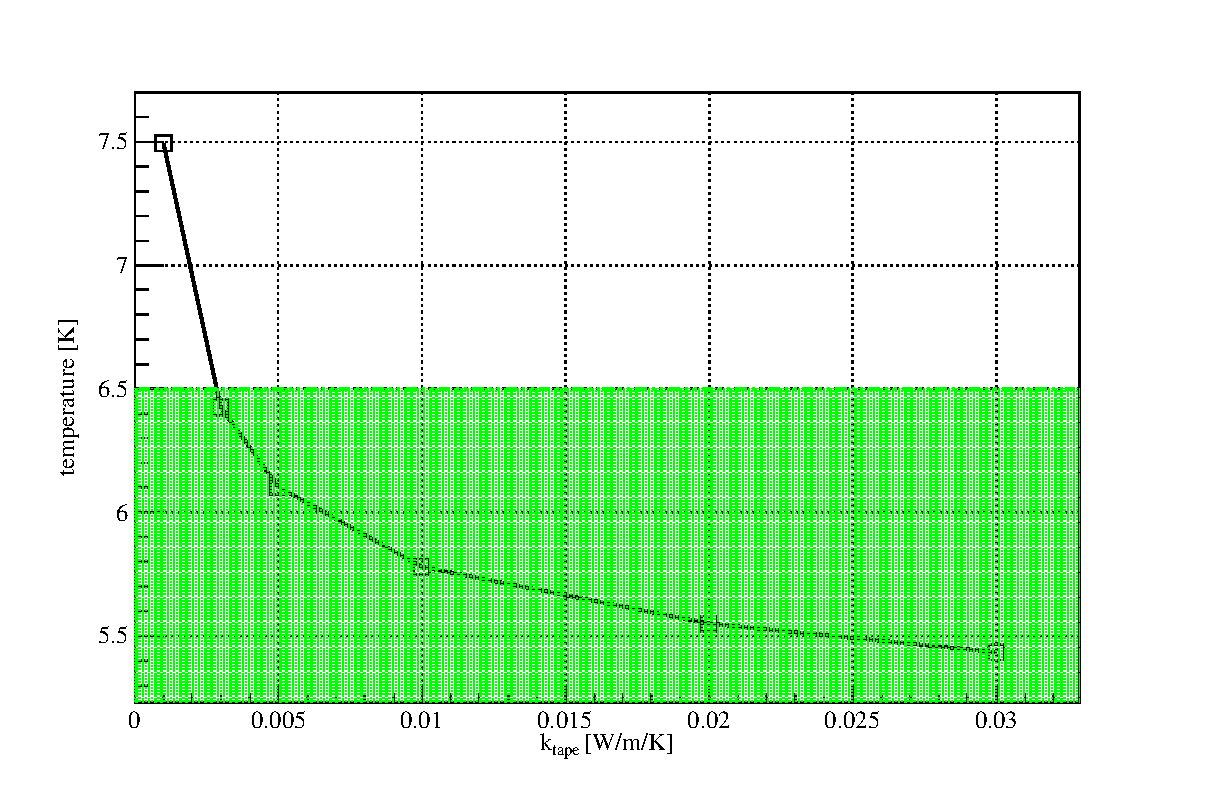
\includegraphics[scale=0.45]{chapter6/fig/tape.eps}
  \caption{ the thermal conductivity dependance of indulation tape.}
  \label{4tape}
 \end{figure}

\subsection{Discussion}
~~~~~~As mentioned in previous chapter, different result of neutron production and energy deposition is obtained in terms of different physics model.
Nowadays' heat calcualtion bases on the model of JAM\_INCL\_JENDL.
We suppose there is fator of $\pm$0.3 in different physics model.
The figure~\ref{5factor} shows the temperature changes with the factor of energy deposition for 90 day operation.
The maximum temperature grows up with factor.
Supposed that the energy deposition predicted by the other physics model is higher than JAM\_INCL\_JENDL by factor 1.5, cooling for 30 days is not allowed for phase-II experiment.
Thus, the energy depostion and neutron production is necessary to be checked correctly by using different physics model in future.
\begin{figure}[H]
 \begin{subfigure}{0.3\textwidth}
 \centering
 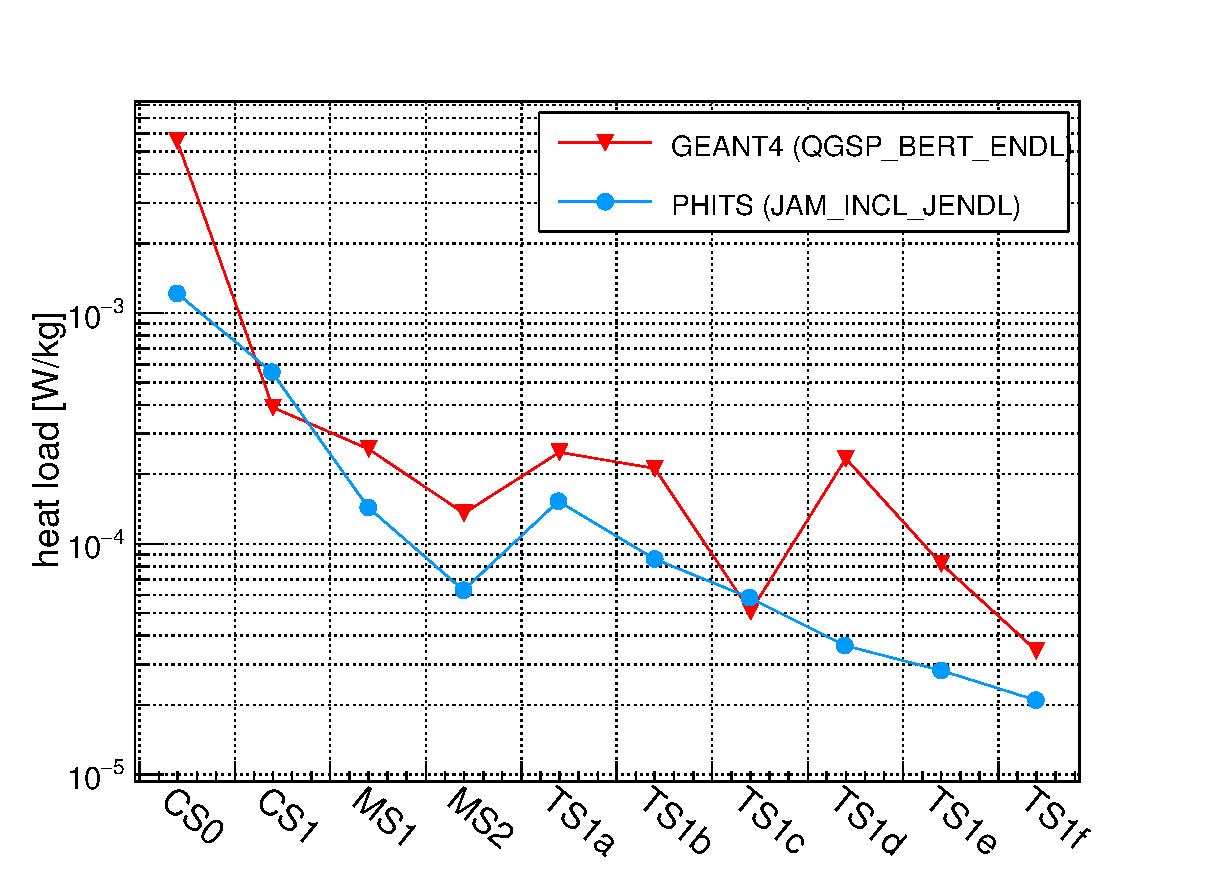
\includegraphics[scale=0.45]{chapter5/fig/g4phs.eps}
 \end{subfigure}
 \hspace{0.2\textwidth}
 \begin{subfigure}{0.3\textwidth}
 \centering
 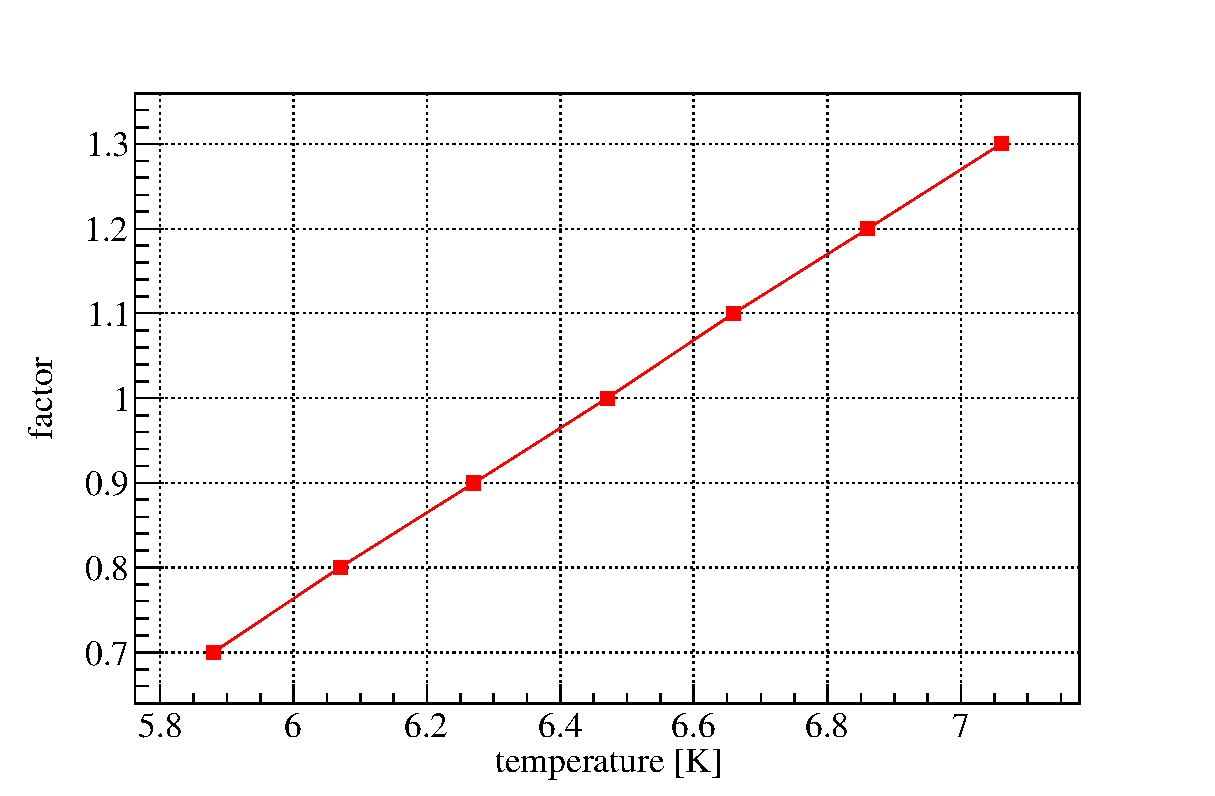
\includegraphics[scale=0.45]{chapter6/fig/factor.eps}
 \end{subfigure}
 \caption{ The temperature peak increases linearly with the energy deposition factor.}
 \label{5factor}
\end{figure}

\subsubsection{Improvement of CS1 coil}
~~~~~~Due to cooling issue of the CS1 coils, the new scenario should be considered if the CS1 cannot be cooled for a long time.
There are two ways to optimize the CS1 coils to enlarge the operating time.
\begin{itemize}
 \setlength{\itemsep}{-5pt}
 \item Using the original design but enlarged the thinckness of aluminium strip.
 \item Seperating the CS1 coils to two parts.
\end{itemize}
As shown in figure~\ref{5opti}, the maximum temperature calculated with 90 day operation is able to be reduced by increasing the thickness of aluminium strip.
If the thickness of aluminium strip can be increased from 1 mm to 2 mm, the peak temperature of 90 day operation is possible to be reduced under current sharing temperature.
However, increasing the thickness of aluminium strip may make the coil winding become difficult.
It still needs to discuss in future.
\begin{figure}[H]
 \centering
 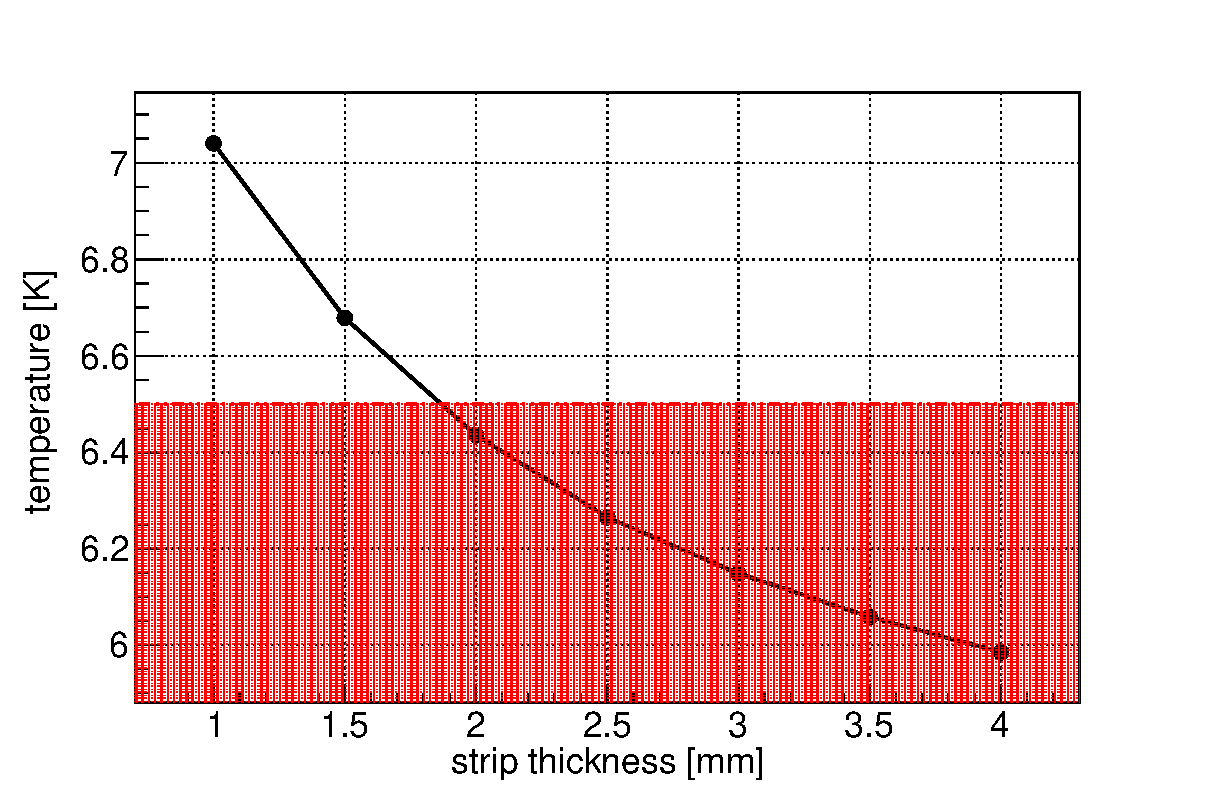
\includegraphics[scale=0.45]{chapter6/fig/Strip.eps}
 \caption{ The CS1 coils can be optimized by imcreasing the thickness of aluminium strip.}
 \label{5opti}
\end{figure}

The second scenario is to seperate the CS1 coils to two parts.
Since the energy deposition peak in the middle of the CS1 coils, seperating the CS1 coils and inserting the aluminium strip in the middle of the CS1 coils, which is shown in figure~\ref{5new}, can help CS1 to be cooled down very well.
\begin{figure}[H]
 \centering
 \includegraphics[scale=0.4]{chapter6/fig/CS1new.pdf}
 \caption{ The scenario of CS1 seperating.}
 \label{5new}
\end{figure}
To validate this scenario, the cooling, quench, magnetic field, muon yield and mechanical issue must be estimated.


